
\chapter{Molla}

\section{Introduzione}
Oggetto di studio è la verifica della legge di Hooke, che lega la deformazione che si manifesta su un corpo soggetto ad una forza elastica all'intensità della forza stessa:
\begin{equation}\label{eq:Hooke}
F=-kx
\end{equation}
Nello specifico delle nostre analisi, ci occuperemo della forza di richiamo di una molla. $x$, che compare nella \ref{eq:Hooke} è l'allungamento della molla dalla posizione di equilibrio.
Noto il valore della forza (nel nostro caso si tratterà sempre della forza peso $F=Mg$), si può inoltre determinare la costante di proporzionalità $k$, caratteristica di ciascuna molla.

\section{Strumenti}
La strumentazione si compone di un gancio cui si appende la molla di cui si vogliono studiare le caratteristiche, e nel punto corrispondente del tavolo (lungo la perpendicolare) si pone un sensore di posizione che trasmette i dati rilevati (allungamento) al computer, dove sono poi analizzati con il programma DataStudio.\\
\\
\begin{tabular}{c c c}
\textbf{Molla A} & \hspace{1.5cm} $L_A=0.430\ m$ & \hspace{1.5cm} $M_A=4.289\ g$\\
\\
\textbf{Molla B} & \hspace{1.5cm} $L_B=0.426\ m$ & \hspace{1.5cm} $M_B=4.029\ g$\\
\end{tabular}
\\
\\
Per la terza parte dell'esperimento ci siamo serviti di un disco di cartone di massa $M=2.5\ g$. 
\\
\\
Con $L_A$ ed $L_B$ si indica la distanza tra il rivelatore e la molla a riposo. 

\section{Misura statica}

La \ref{eq:Hooke} implica che il rapporto tra l'allungamento della molla e la forza esercitata sia un valore costante:
$$k=\frac{Mg}{x}$$
Facendo variare le masse appese, verifichiamo dunque la validità della \ref{eq:Hooke} e successivamente otteniamo il valore di $k_1$ e $k_2$ corrispondenti alle due molle.   
Di seguito in tabella i valori raccolti per le due molle, ottenuti dal rivelatore di distanza. \footnote{I valori sono stati raccolti con una frequenza di campionamento di 10 $Hz$}
\footnote{Durante tutto l'esperimento gli errori associati alle interpolazioni si sono rivelati trascurabili (dell'ordine di $10^{-5}$ i più grandi), per cui ne abbiamo evitato anche la trascrizione.}

\begin{center}

\begin{tabular}{c c}
\textbf{Molla A} & \hspace{2cm} \textbf{Molla B}\\
\\
\begin{tabular}{c|c|c}
Massa ($kg$) & Misura L ($m$) & $\Delta L$ ($m$)\\
\midrule
0.200 & 0.422 & 0.008\\
0.250 & 0.420 & 0.010\\
0.300 & 0.418 & 0.012\\
0.400 & 0.414 & 0.016\\
0.450 & 0.412 & 0.018\\
0.500 & 0.410 & 0.020\\
0.550 & 0.408 & 0.022\\
0.600 & 0.406 & 0.024\\
0.650 & 0.404 & 0.026\\
0.700 & 0.402 & 0.028\\
\end{tabular}

& \hspace{2cm}

\begin{tabular}{c|c|c}
Massa ($kg$) & Misura L ($m$) & $\Delta L$ ($m$)\\
\midrule
0.200 & 0.424 & 0.002\\
0.250 & 0.422 & 0.004\\
0.300 & 0.420 & 0.006\\
0.400 & 0.416 & 0.010\\
0.450 & 0.413 & 0.013\\
0.500 & 0.411 & 0.015\\
0.550 & 0.409 & 0.017\\
0.600 & 0.407 & 0.020\\
0.650 & 0.404 & 0.022\\
0.700 & 0.402 & 0.024\\
\end{tabular}
\\
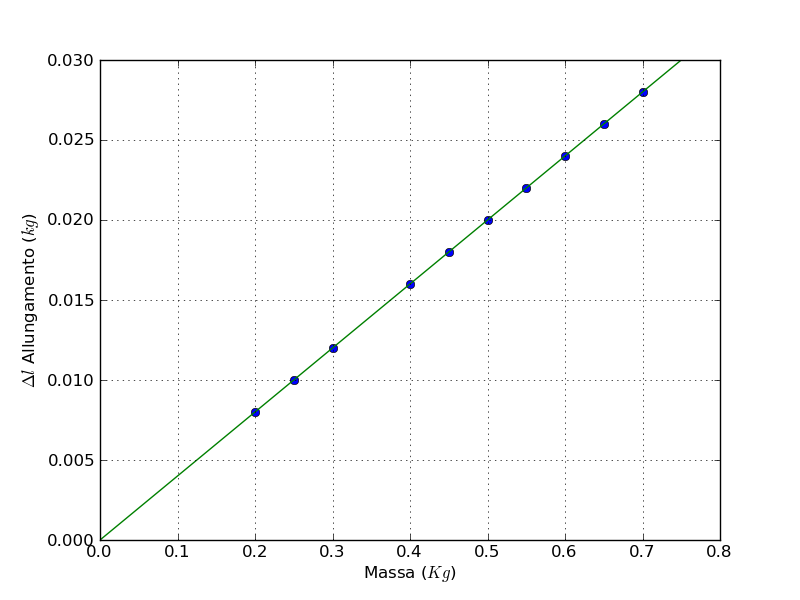
\includegraphics[scale=0.4]{../grafici/molla/mollaAstatica} & \hspace{1cm}
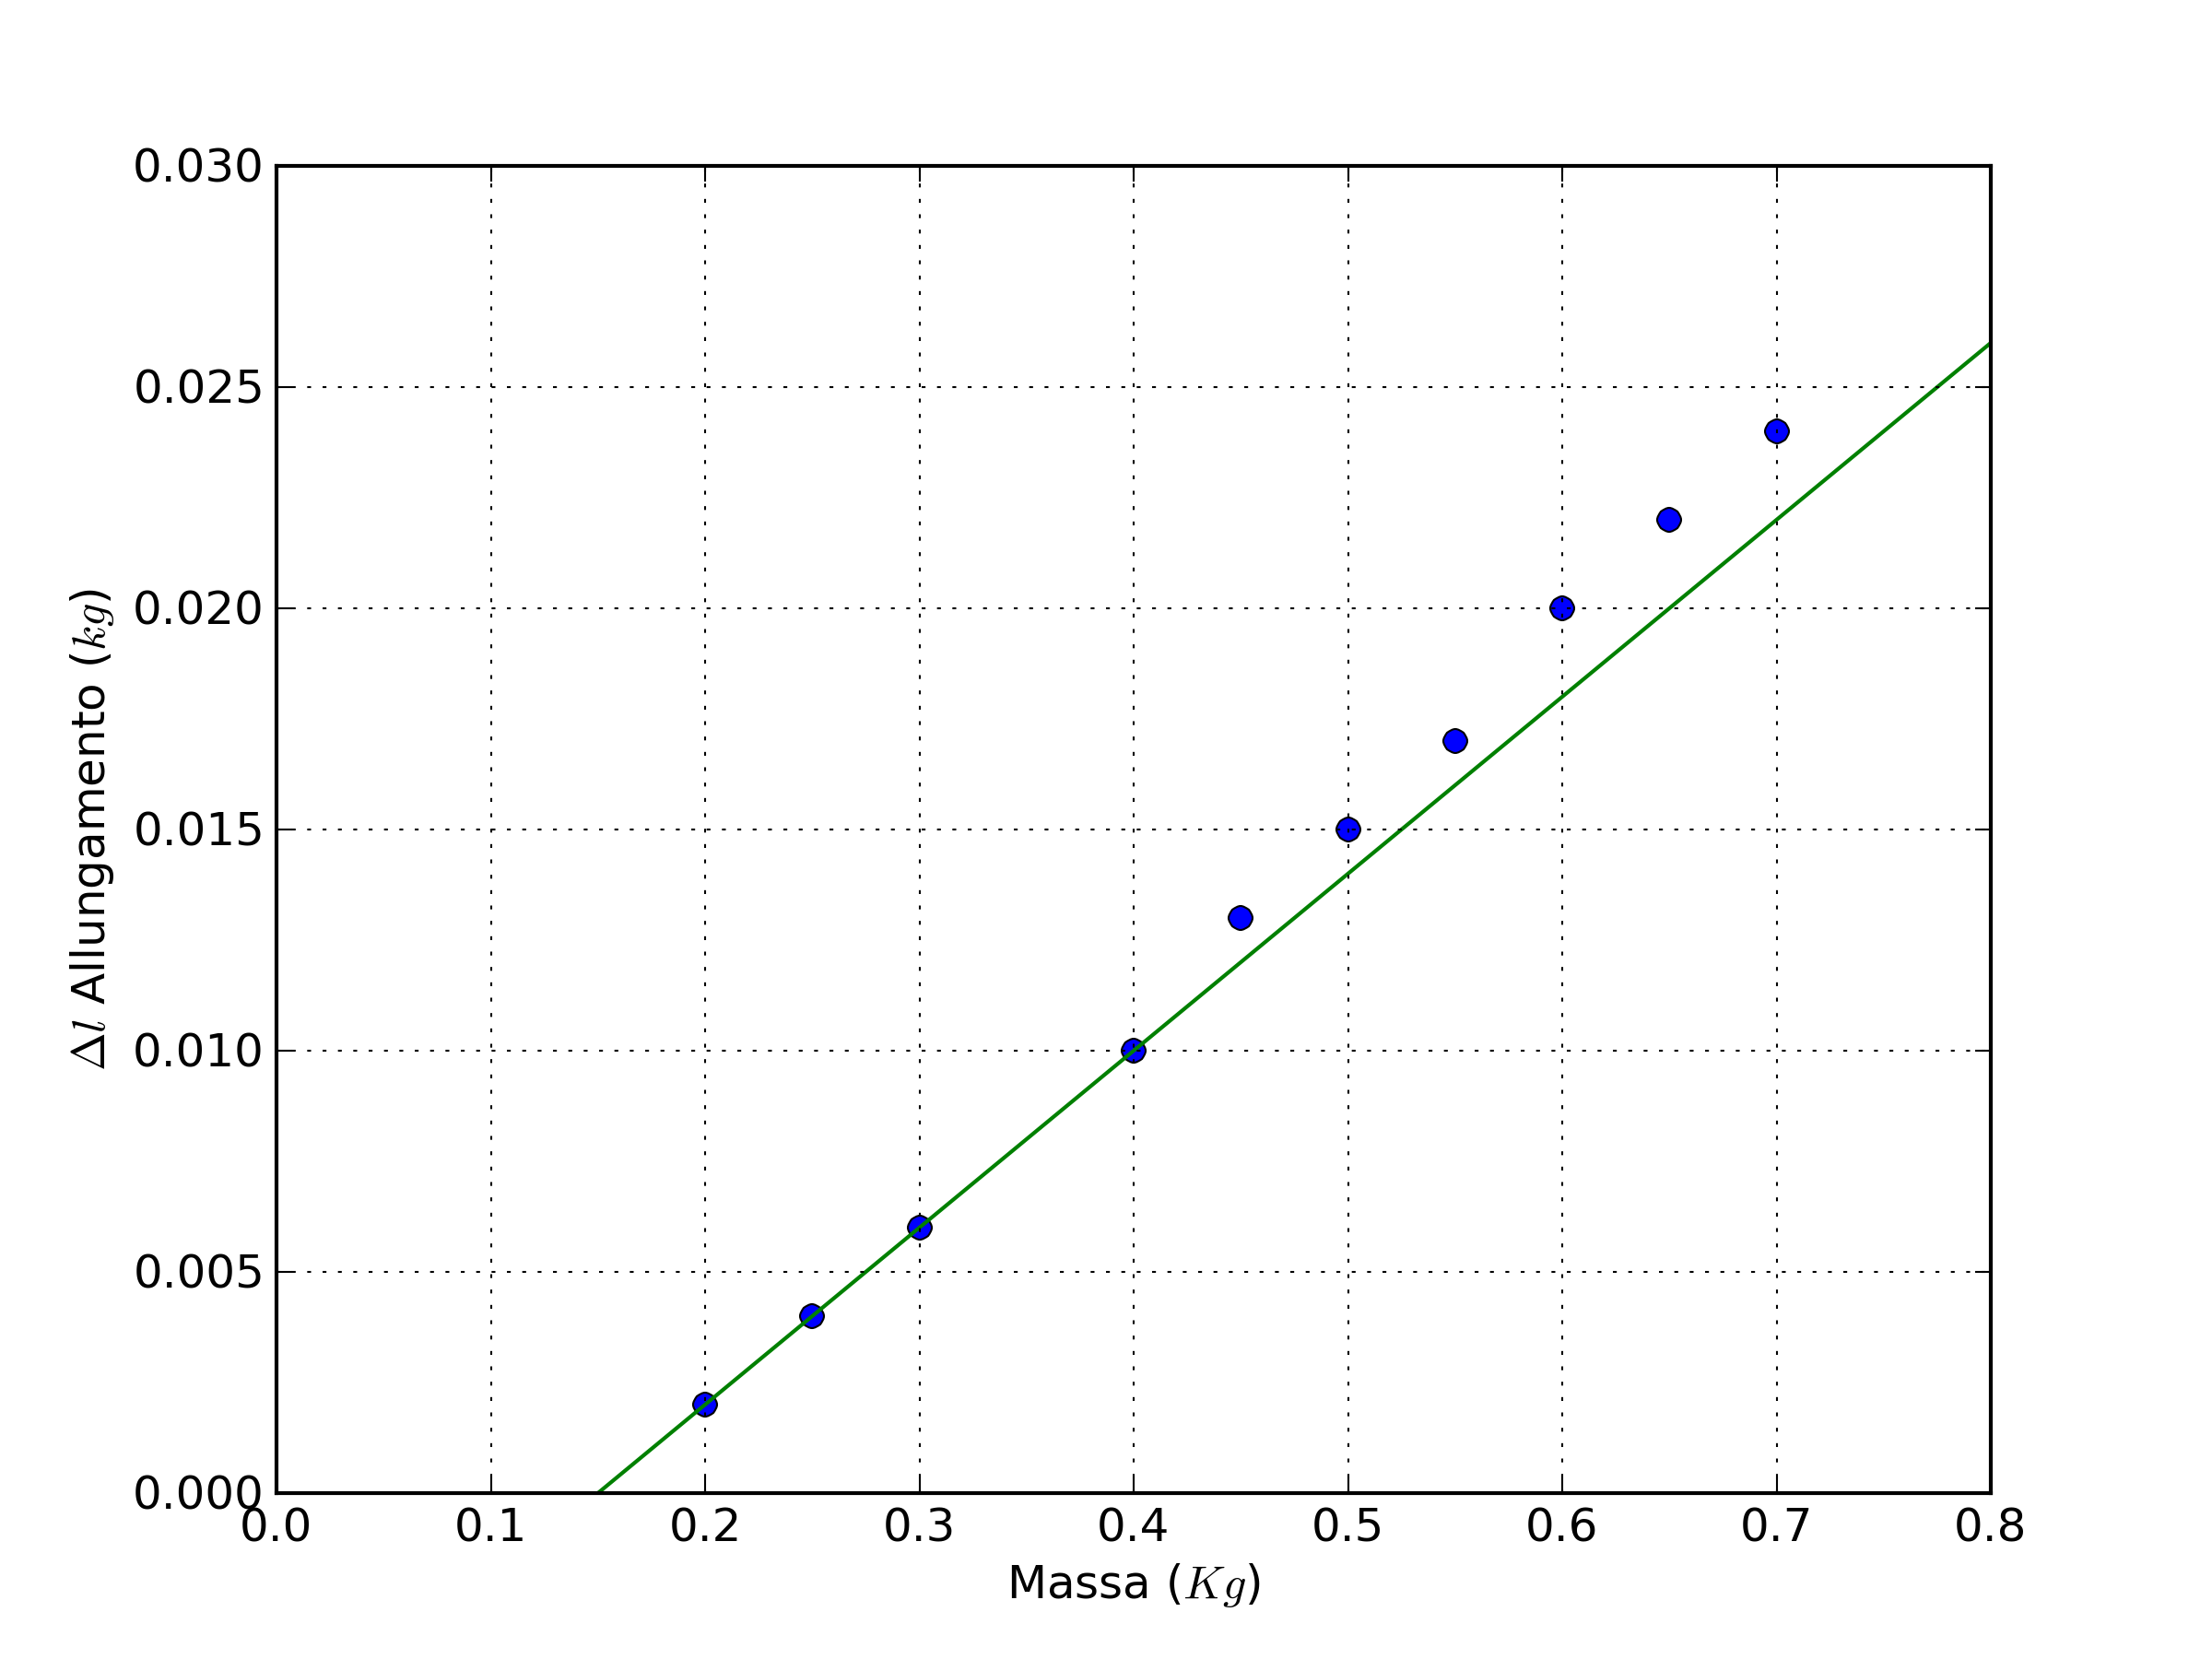
\includegraphics[scale=0.4]{../grafici/molla/mollaBstatica}\\
$P(\tilde{\chi}^2\geq\tilde{\chi_0}^2) \simeq 6,3\%$&\hspace{1cm}$P(\tilde{\chi}^2\geq\tilde{\chi_0}^2) \simeq 1,1\%$
\footnote{Avendo fissato un livello di confidenza del 5 \% , questa distribuzione va rigettata.}\\

\end{tabular}


\end{center}



\section{Misura dinamica}

\subsubsection{Procedimento e breve accenno di teoria}

Quando una molla viene spostata dalla propria posizione di equilibrio, essa esercita una forza di richiamo data dalla \ref{eq:Hooke}. Se su di essa agisce anche la forza peso, si ha:
$$\displaystyle\sum{F}=Mg-kx$$
Dalla II legge di Newton, dividendo tutto per M ed esprimendo $g$ dalla \ref{eq:Hooke} come $g=\displaystyle{\frac{kx_0}{M}}$, ricaviamo:

\begin{equation}
\frac{d^2x}{dt^2}+\frac{k}{M}(x-x_0)
\end{equation}

con $x_0=\displaystyle{\frac{Mg}{k}}$ posizione di equilibrio.\\
\\
Tale equazione descrive un moto armonico semplice, la cui legge del moto è data da:

\begin{equation}\label{eqmoto}
x(t)=x_0+Asin(\omega t+\phi)
\end{equation} 
il cui periodo, nel caso di molle con massa non trascurabile, è dato da:

\begin{equation}\label{periodo}
T=2\pi\sqrt{\frac{M+m/3}{k}}
\end{equation}  

con $m$ massa della molla. A questo punto è facile determinare il valore di $k$. Sospendiamo dunque alla molla una massa, e discostatala dalla posizione di equilibrio la lasciamo libera di oscillare. Verifichiamo dal grafico tracciato in tempo relale dal programma DataStudio, sincronizzato alla fotocellula di posizione, che si tratti effettivamente di un moto armonico. Infine dai valori del quadrato del periodo, ottenuti mediante l'interpolazione con una sinusoidale, si ricava il valore di $k$. In questo caso si fa uso di una interpolazione con il metodo dei minimi quadrati, ponendo $x_i=M_i$, $y_i={T_i}^2$ ed $m=\displaystyle{\frac{4\pi^2}{k}}$. 

\subsubsection{Raccolta dati}

\begin{center}

\begin{tabular}{c c}
\textbf{Molla A} & \hspace{2cm} \textbf{Molla B}\\
\\
\begin{tabular}{c | c| c}
Massa ($g$) & Periodo ($s$) & Pulsazione ($rad/s$)\\
\midrule
400 & 0.274 & 22.93\\
600 & 0.340 & 18.48\\
800 & 0.374 & 16.80\\
\end{tabular}

& \hspace{2cm}

\begin{tabular}{c | c | c}
Massa ($g$) & Periodo ($s$) & Pulsazione ($rad/s$)\\
\midrule
500 & 0.312 & 20.14\\
700 & 0.364 & 17.26\\
900 & 0.409 & 15.36\\
\end{tabular}
\\
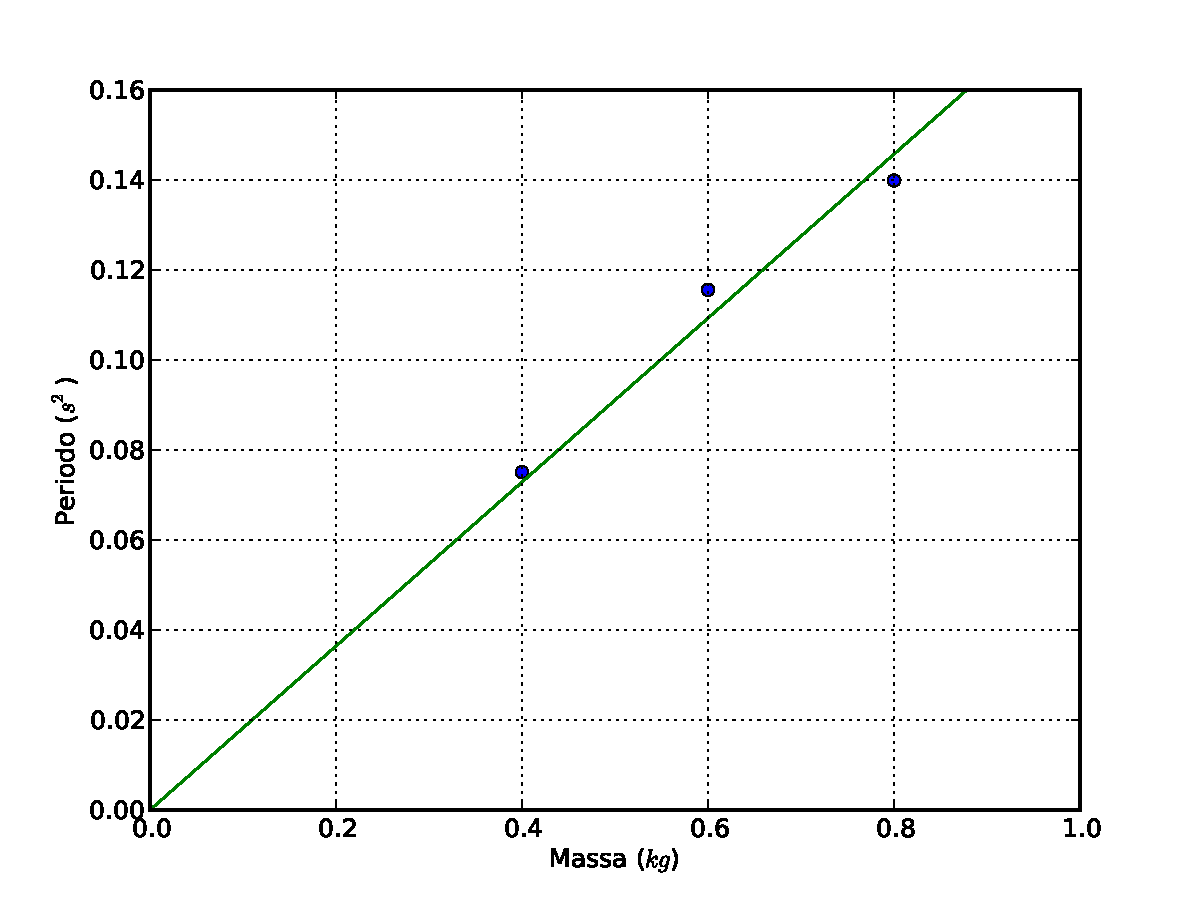
\includegraphics[scale=0.4]{../grafici/molla/mollaA.pdf}& \hspace{1cm}
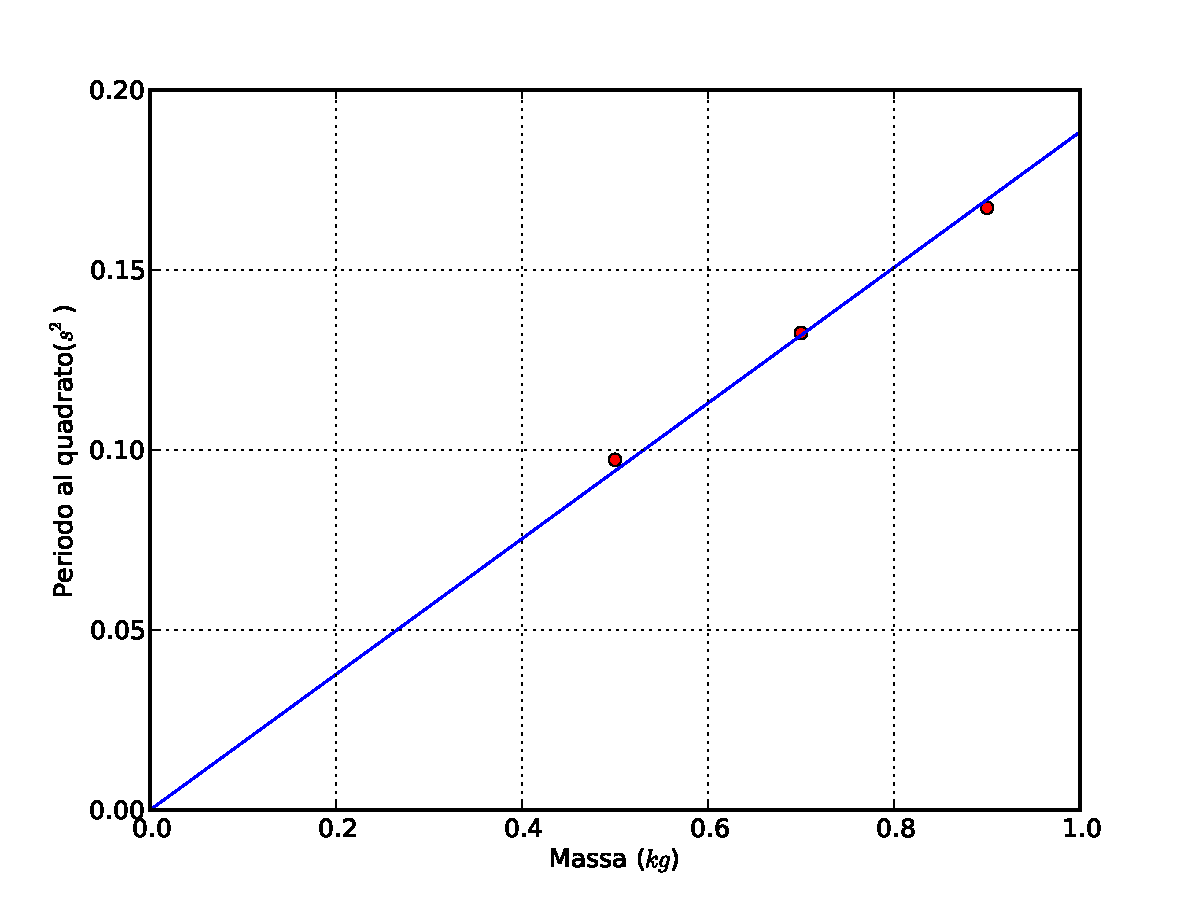
\includegraphics[scale=0.4]{../grafici/molla/mollaB.pdf}\\
\end{tabular}

\end{center}

I grafici mostrano la dipendenza lineare tra $T^2$ ed $M$.


Dall'interpolazione ricaviamo:
\begin{center}
\begin{tabular}{c c}
$m_A=0.182$ & \hspace{3cm} $m_B=0.188$\\ 
\\
$k_A=\displaystyle{\frac{4\pi^2}{m_A}}=216.9\ Nm$ & \hspace{3cm} $k_B=\displaystyle{\frac{4\pi^2}{m_B}}=210.0\ Nm$ \\
\end{tabular}

\end{center}

Dal calcolo del $\chi^2$, otteniamo  $\chi^2_{a} = 162$ e $\chi^2_{b} = 35$. Entrambi i  $\chi^2$ sono molto maggiori del numero delle misure. Il disaccordo dai dati è quindi significativo e siamo costretti a rigettare le nostre distribuzione. 

Proviamo ad interpolare i dati con una funzione lineare del tipo $y = Bx+A$. 
\begin{center}
\begin{tabular}{c c}
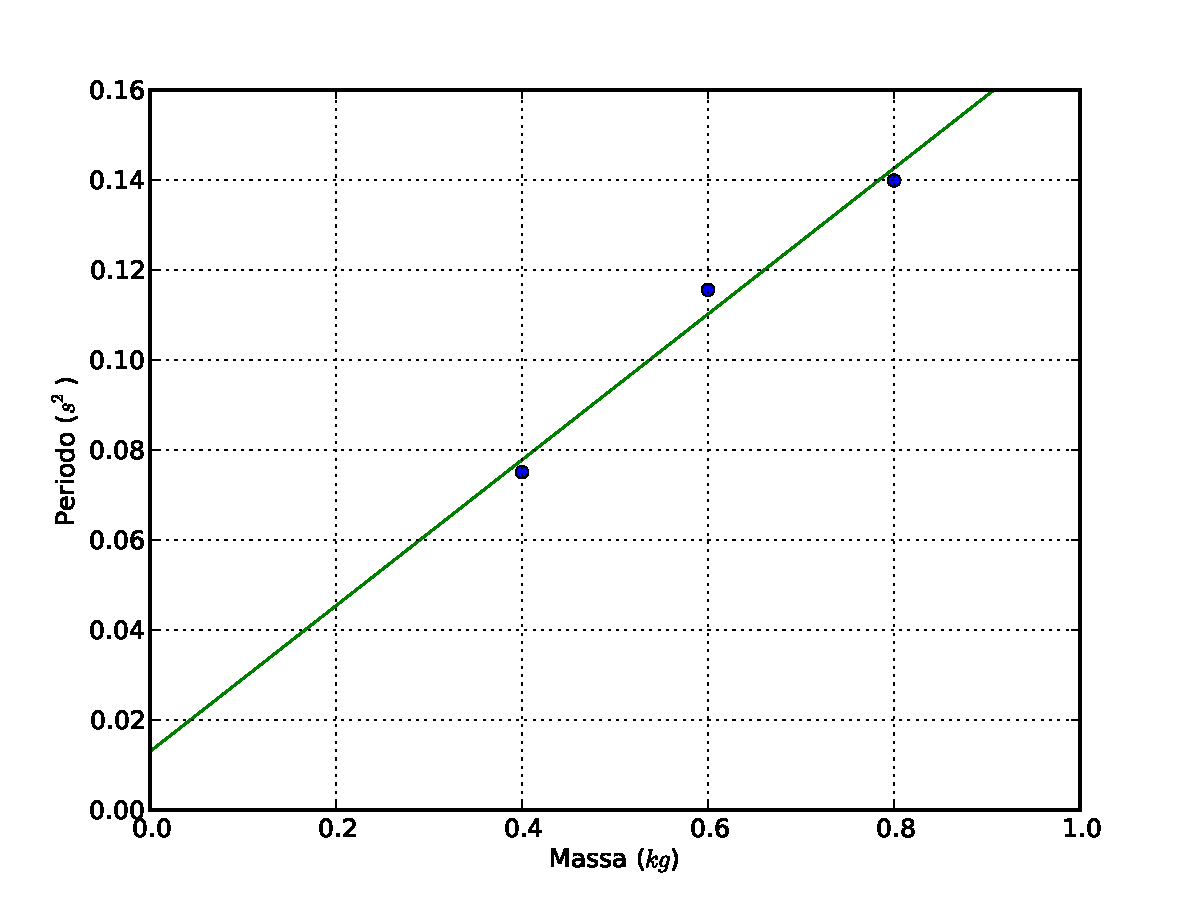
\includegraphics[scale=0.4]{../grafici/molla/mollaAsecondo.pdf}&\hspace{1cm}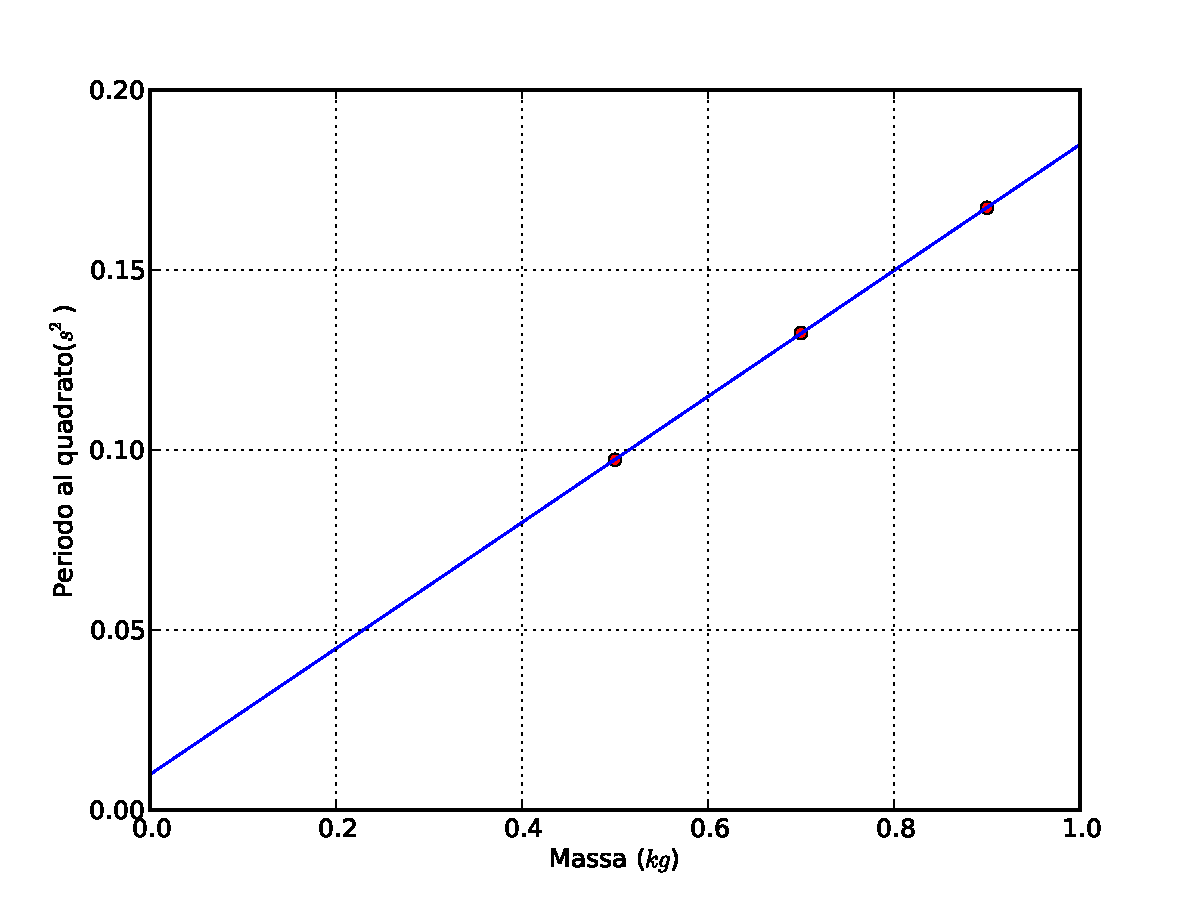
\includegraphics[scale=0.4]{../grafici/molla/mollaBsecondo.pdf}\\

\end{tabular}
\end{center}

L'accordo per la molla B aumenta in maniera significativa. Il $\chi^2$ ha un valore di $0.04$, vi è quindi accordo tra i dati e l'interpolazione scelta.
La presenza di un intercetta sull'asse $y$, che non è presente nella relazione lineare teorica, può essere dovuta ad un errore sistematico nella misurazione, come ad esempio una  calibrazione non corretta. 

\section{Moto armonico smorzato}

Fissando il disco di cartone all'estremità oscillante della molla, si aumenta l'effetto frenante dell'aria ($F=-bv$, con $b$ coefficiente di smorzamento).  
In tal caso si assiste ad una diminuzione dell'ampiezza di oscillazione, secondo la legge:
\begin{equation}\label{Asm}
A(t)=A_{max}exp[-b/2M)t]
\end{equation}
E la legge del moto diventa:
\begin{equation}
x(t)=A(t)\cos(\omega't-\phi)=A_{max}exp[-(b/2M)t]\cos(\omega't-\phi)
\end{equation}
con $\omega'^2=\omega^2-(b/2M)^2$.

Utilizziamo tale funzione per interpolare i dati e ricavare il valore della costante $b$, al variare di M.\footnote{I dati sono stati raccolti con una frequenza di campionamento di 40 $Hz$}
\begin{center}

\begin{tabular}{c c}
\textbf{Molla A} & \hspace{1cm} \textbf{Molla B}\\
\\
\begin{tabular}{c | c | c | c}
$\boldsymbol{M}$ ($kg$) & $\boldsymbol{T}$ ($s$) & $\boldsymbol{\omega'}$ ($rad/s$) & $\boldsymbol{b}$ ($kg/s$)\\
\midrule
0.400 & 0.284 & 22.113 & 0.0228\\
0.600 & 0.336 & 18.690 & 0.0329\\
0.800 & 0.381 & 16.483 & 0.0369\\
\end{tabular}

& \hspace{1cm}

\begin{tabular}{c | c | c | c}
$\boldsymbol{M}$ ($kg$) & $\boldsymbol{T}$ ($s$) & $\boldsymbol{\omega'}$ ($rad/s$) & $\boldsymbol{b}$ ($kg/s$)\\
\midrule
0.500 & 0.321 & 19.574 & 0.0262\\
0.900 & 0.416 & 15.096 & 0.0364\\
0.700 & 0.372 & 16.882 & 0.0291\\
\end{tabular}

\end{tabular}

\end{center}

\begin{center}

\begin{tabular}{c c}
$\bar{b}_A=\displaystyle{\frac{\sum{b_i}}{N}}=0.0309\ kg/s$ & \hspace{1cm} $\bar{b}_B=\displaystyle{\frac{\sum{b_i}}{N}}= 0.0306\ kg/s$\\
\\
$\sigma_{\bar{b}_A}=\displaystyle{\sqrt{\frac{\sum{(b_i-\bar{b})^2}}{N-1}}}=0.0073\ kg/s$ & \hspace{1cm} $\sigma_{\bar{b}_B}=\displaystyle{\sqrt{\frac{\sum{(b_i-\bar{b})^2}}{N-1}}}= 0.0053\ kg/s$\\
\end{tabular}

\end{center}

È inoltre possibile ricavare $\omega'$ direttamente dal periodo delle oscillazioni smorzate: confrontiamo i valori ottenuti con i due differenti metodi:

\begin{center}

\begin{tabular}{c c}
\textbf{Molla A} & \hspace{2cm} \textbf{Molla B}\\
\\
\begin{tabular}{c | c}
$\boldsymbol{\omega'_{interpolato}}$ ($rad/s$) & $\boldsymbol{\omega'_{calcolato}}$ ($rad/s$)\\
\midrule
22.113 & 22.123\\
18.690 & 18.699\\
16.483 & 16.491\\
\end{tabular}

& \hspace{1cm}

\begin{tabular}{c | c}
$\boldsymbol{\omega'_{interpolato}}$ ($rad/s$) & $\boldsymbol{\omega'_{calcolato}}$ ($rad/s$)\\
\midrule
19.574 & 19.573\\
15.096 & 15.103\\
16.882 & 16.890\\
\end{tabular}

\end{tabular}

\end{center}